% ----------------------------------------------------------
% Revisão bibliográfica
% ----------------------------------------------------------
\chapter{Revisão da literatura}
\label{chp:revisão}

\marcos{Explique melhor as soluções: você tem espaço, então pode deixar este capítulo muito mais auto-contido}

Existem vários aspectos relativos à análise forense na nuvem, indo desde a coleta de informações até a garantia da cadeia de custódia de evidências.
%
Das propostas encontradas em literatura 6 foram selecionadas como melhor representação do estado da arte, a seguir uma breve descrição de cada uma delas.

%
O modelo proposto por \cite{ReichertAutoAcquisition:2015} é um processo de coleta de evidências integrado ao \textit{hypervisor} e disparado por algum sistema de detecção de intrusão. 
%
A partir do momento em que uma ameaça é detectada, o modelo tira instantâneos das máquinas virtuais comprometidas. O modelo toma cuidado para exclui informações de clientes não relacionados a investigação e armazena o restante em local seguro, tudo de forma automatizada. 
%
O modelo faz uso de GRR para agregar e analisar as evidências coletadas e caso alguma delas case com ameaças armazenadas conhecidas ele alerta um usuário humano para uma avaliação mais detalhada.
%
O intevalo de tempo em que os instantâneos de memória são gerados é configurável e são todos armazenados em persistência.
%
Este modelo tem como principal vantagem a automação do processo de coleta, sem interevenção humana é mais fácil garantir a cadeia de custódia. 
%
A figura \ref{fig:ReichertAutoAcquisitionModel} mostra o desenho da arquitetura proposta pelo autor.

\begin{figure}[htb!]
\footnotesize
\caption{Automated Forensics Data Acquisition Model}
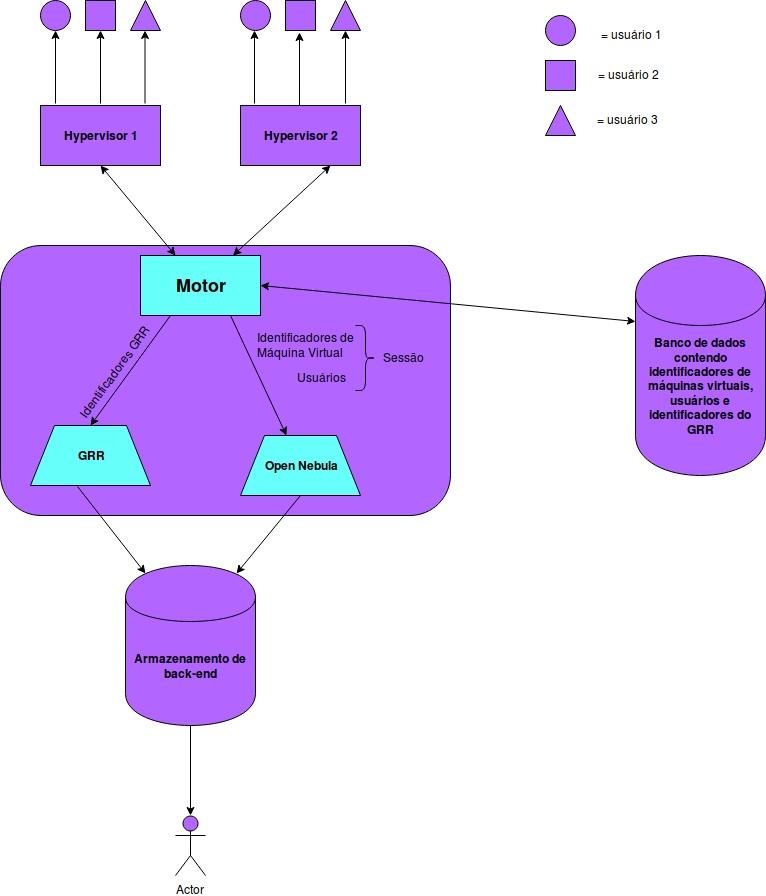
\includegraphics[scale=0.30]{ReichertAutoAcquisitionModel.png}
\centering
\label{fig:ReichertAutoAcquisitionModel}
\begin{center}
Fonte: \cite{ReichertAutoAcquisition:2015} 
\end{center}
\end{figure}

A proposta de \cite{PoiselVMI:2013} é baseada na técnica de introspecção em máquina virtual (VMI) para coleta de memória volátil. 
%
Esta técnica se apoia na necessidade do gerenciador de máquinas virtuais (VMM) em conseguir mapear recursos físicos da máquina hospedeira a recursos alocados à máquina virtual cliente.
%
Este mapeamento também permite que a memória volátil copiada da máquina virtual seja reconstruida em uma máquina física para realização da análise.
%
A proposta utiliza de coleta continua dos instantâneos de memória durante o funcionamento do sistema sem distinção do que aconteceu antes ou depois do fato de interesse.
%
Todos os instantâneos de memória são armazenados para posterior análise.
%
Para eliminar a chance de inconsistências no instantâneo de memória volátil, a máquina virtual tem sua execução suspensa durante o processo de extração.
%
Uma desvantagem da técnica de VMI mencionado pelo próprio autor é a necessidade de tradução de endereços de memória da máquina virtual em endereços de memória da máquina física hospedeira.
%
Esta tradução depende de conhecimento do que está sendo executado na máquina virtual, logo uma solução baseada em VMI não é completamente portável sendo necessário adequações para diferentes clientes além de ser computacionalmente custoso.
%

O framework proposto por \cite{SangLogApproach:2013} é um sistema que funciona em parceria com o provedor de nuvem onde este último envie informações ao framework que os armazena em um local centralizado.
%
O conjunto de informações armazenadas é acordado antecipadamente com o provedor de nuvem e vão desde instantâneos de memória volátil até pacotes trafegados nas interfaces de rede da máquina virtual.
%
O framework coleta informações continuamente e usa cálculo de hash das evidências enviadas pelo provedor de nuvem para garantir que as mesmas não foram alteradas durante o transporte.
%
Assim como as propostas anteriores, esta tambem não faz distinção do que aconteceu antes ou depois do fato de interesse coletando constantemente informações da máquina virtual.
%
O próprio autor menciona que o framework tem a desvantagem de depender da cooperação do provedor de nuvem, uma estratégia considerada fraca pela comunicade pois a prioridade do CSP é o de garantir a disponibilidade do serviço não o de coletar evidências \cite{ClarkeReviewOfChallenges2015}.
%
A figura \ref{fig:SangLogApproach} mostra um esquema do funcionamento da solução focada em um caso específico de log de rede como proposta pelo autor.

\begin{figure}[htb!]
\footnotesize
\caption{A Log Based Approach Model}
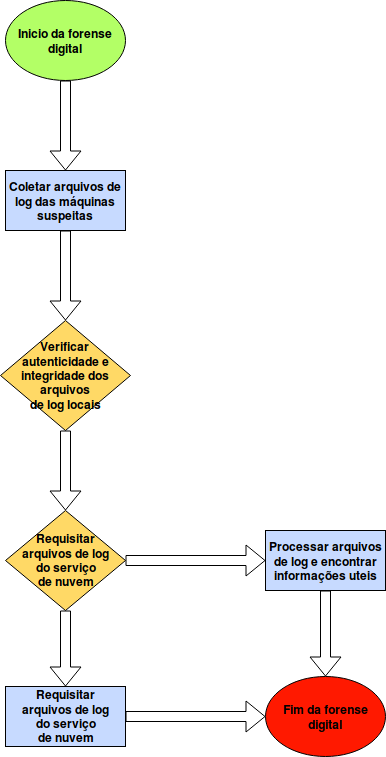
\includegraphics[scale=0.50]{SangLogApproach.png}
\centering
\label{fig:SangLogApproach}
\begin{center}
Fonte: \cite{SangLogApproach:2013} 
\end{center}
\end{figure}

O trabalho descrito em \cite{DezfouliBackupApproach:2012} é voltada a dispositivos móveis e demonstra preocupação com as limitações de armazenamento do dispositivo.
%
O processo de coleta de informações de memória volátil é feita continuamente independente de eventos de interesse como detecção de ameaças.
%
O processo de coleta do instantâneo de memória volátil do dispositivo separa as informações e as armazena por processo ativo, o autor usa esta técnica para melhor gerenciar o espaço que as informações estão ocupando em disco. 
%
Possui inteligência para descartar informações de processos que foram terminados e removidos da memória assim como inteligência para fazer uso ótimo do espaço de armazenamento do device.
%
A figura \ref{fig:DezfouliBackupApproach} o autor mostra um esquema macro de como o armazenamento da evidência é gerenciado.

\begin{figure}[htb!]
\footnotesize
\caption{Backup Approach Model}
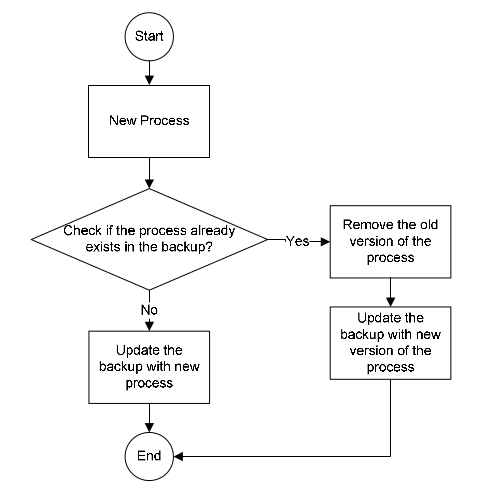
\includegraphics[scale=0.50]{DezfouliBackupApproach.png}
\centering
\label{fig:DezfouliBackupApproach}
\begin{center}
Fonte: \cite{DezfouliBackupApproach:2012} 
\end{center}
\end{figure}

A ferramenta FROST proposto por \cite{DykstraFROST:2013} descreve um conjunto de bibliotecas integradas aono arcabouço \textit{Open Stack Framework} de gerenciamento de infra estruturas virtualizadas.
%
Através desta integração, FROST expõe um conjunto de API para serem usadas por aplicações de coleta de evidências forenses que dão acesso a recursos da máquina virtual sendo administrada como disco, logs de trafego de rede, e memória volátil.
%
A proposta descreve apenas o arcabouço, deixa a critério do usuário detalhes como periodicidade e tamanho da coleta assim como onde a evidência será armazenada.
%
De todas as propostas descritas neste capítulo esta é a única que demonstra preocupação com adequação a questões legais e padrões já estabelecidos na industria forense.
%
O autor declara que FROST segue as práticas definidas no Grupo de Trabalho Sobre Evidência Digital (SWGDE) e do Manual de Busca em Apreensão do Departamento de Justiça Norte-Americano.
%
A figura \ref{fig:DykstraFROST} o autor mostra um esquema macro da integração entre FROST e o arcabouço \textit{Open Stack Framework}

\begin{figure}[htb!]
\footnotesize
\caption{FROST}
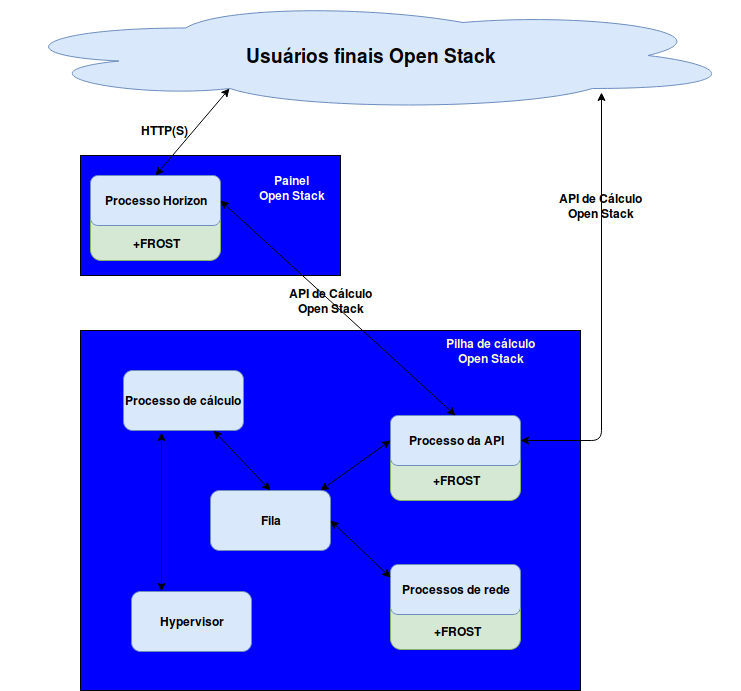
\includegraphics[scale=0.50]{DykstraFROST.png}
\centering
\label{fig:DykstraFROST}
\begin{center}
Fonte: \cite{DykstraFROST:2013} 
\end{center}
\end{figure}
%

O trabalho descrito em \cite{GeorgeDF2CE:2012} está focado em monitoração de rede e opera em uma arquitetura de forense como serviço (FaaS). 
%
O autor propõe um conjunto de ferramentas que tem capacidade de realizar auto descoberta das interfaces que devem ser monitoradas, coletar evidências de tais máquinas e armazena-las.
%
O processo de auto descoberta e associação das evidências com usuários de rede é realizado por um motor baseado em ontologias armazenadas em um banco de dados próprio.
%
Na figura \ref{fig:GeorgeDF2CE} mostra o desenho da aquitetura proposta pelo autor.

\begin{figure}[htb!]
\footnotesize
\caption{Digital Forensic Framework for Cloud Environment}
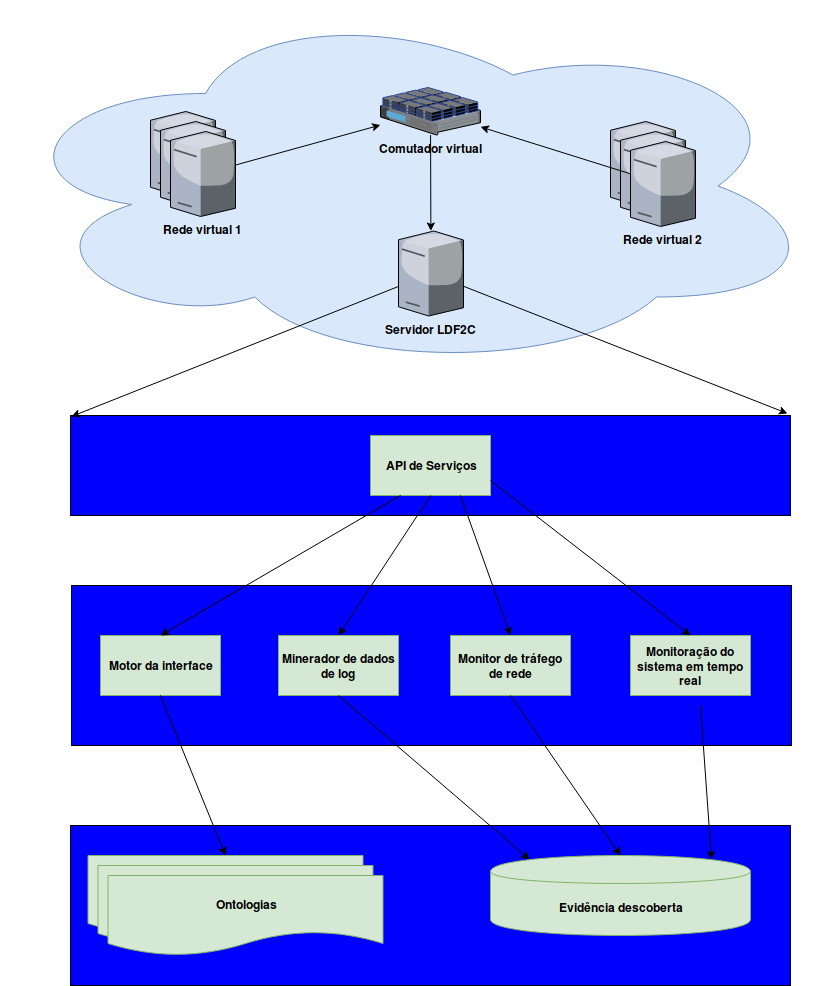
\includegraphics[scale=0.50]{GeorgeDF2CE.png}
\centering
\label{fig:GeorgeDF2CE}
\begin{center}
Fonte: \cite{GeorgeDF2CE:2012} 
\end{center}
\end{figure}

A seguir os trabalhos mencionados acima são agrupados e avaliados com base nos diferentes aspectos que abordam.

\section{Acessar e coletar as informações de memória das máquinas virtuais em nuvem}
\label{sec:coletadeevidencia}

Diversos trabalhos de análise forense na nuvem se concentram na coleta de dados ``após o fato'', ou seja, após a intrusão ser detectada \cite{ReichertAutoAcquisition:2015,PoiselVMI:2013,DykstraFROST:2013,GeorgeDF2CE:2012,SangLogApproach:2013}. 
%
Os processos de coleta descritos nesses trabalhos podem ser iniciados de forma manual ou automaticamente, via integração com um mecanismo de detecção de intrusão. 
%
No caso específico de memória volátil, tal forma de coleta não consegue descrever como era a memória antes da intrusão, pois o processo só é acionado depois da detecção do ataque. 
%
%A capacidade de saber como era a memória antes do fato é descrita por \cite{Case_Memory_Forensics:2014} como necessária para viabilizar a abordagem de coletar o suficiente para realizar a investigação pois permite comparar dois instantâneos de memória e minimizar o volume coletado antes do fato. 
Tal limitação pode trazer prejuízos à investigação, dado que algumas análises dependem exatamente da capacidade de se comparar dois momentos da memória \cite{CaseMemoryForensics:2014}. 
%
Entre os trabalhos estudados, a única proposta encontrada que leva tal necessidade em consideração é \cite{DezfouliBackupApproach:2012}, que propõe que o dado seja armazenado no próprio equipamento sob análise.
%
%Infelizmente, entretanto, essa abordagem não é aplicável ao cenário em nuvem, pois leva a perda de informações importantes caso a máquina virtual seja despejada e seus recursos liberados.
Infelizmente, entretanto, a aplicação de tal abordagem no cenário em nuvem é pouco viável, pois pode levar à perda de informações importantes caso a máquina virtual ou contêiner seja desativada, tendo seus recursos liberados.
%

%Ainda na coleta de informações, os autores \cite{Reichert_Auto_acquisition:2015} e \cite{George_DF2CE:2012} sugerem a abordagem de forense ao vivo onde os dados são constantemente coletados sem distinção do antes ou depois do fato. 
Existem ainda trabalhos voltados à coleta de informações durante a execução do sistema, nos quais os dados são constantemente coletados sem distinção do que aconteceu antes ou depois do fato de interesse.
%
Esse é o caso de trabalhos como \cite{PoiselVMI:2013,DykstraFROST:2013,SangLogApproach:2013}, que adotam a estratégia de isolar e parar a máquina virtual para em seguida realizar o processo de coleta. 
%
%Nas duas estratégias citadas anteriormente, o problema do grande volume de informações coletadas não é abordado pelo autores nem o cenário onde é necessário coletar evidências de uma máquina virtual que já foi despejada do pool e os recursos liberados. 
Embora interessantes, as abordagens descritas nesses trabalhos podem levar a um elevado volume de dados coletados, além de também não tratarem o cenário em que é necessário coletar evidências quando os recursos virtuais contendo tais informações são liberados.


\section{Capacidade de reproduzir o processo e obter os mesmos resultados}
\label{sec:reprodutibilidade}

Se, durante uma análise forense, analistas diferentes obtêm resultados distintos ao executar o mesmo procedimento de coleta, a evidência gerada não tem credibilidade, inviabilizando seu uso em um processo legal. 
%
Por essa razão, a reprodutibilidade do processo de coleta é uma parte importante da geração de evidências para análise forense.
%
Infelizmente, entretanto, nenhuma das propostas encontradas na literatura atualmente permite tal reprodutibilidade em cenários de nuvem em que máquinas virtuais ou contêineres são desativados e seus recursos físicos liberados: todas elas dependem da existência do recurso virtual para a repetição do processo de coleta.

\section{Não violar privacidade ou jurisdição das partes não envolvidas na investigação}
\label{sec:legais}

Em um ambiente de nuvem pública, remover o \textit{hardware} para análise posterior pode levar à violação de privacidade de usuários, uma vez que o multi-inquilinato desse cenário faz com que uma mesma máquina física guarde informações de diversos clientes, alguns dos quais podem não estar envolvidos na investigação em curso.
%
Diversos trabalhos na literatura tratam esse problema adequadamente, por meio das duas estratégias principais: a primeira, adotada em \cite{ReichertAutoAcquisition:2015,GeorgeDF2CE:2012,PoiselVMI:2013,DykstraFROST:2013}, consiste em coletar dados pertinentes à investigação e armazená-los fora da nuvem; a segunda, empregada em \cite{SangLogApproach:2013} e que constitui um caso específico de \cite{GeorgeDF2CE:2012}, depende da cooperação do provedor de serviços de nuvem para conseguir as informações necessárias à investigação. 
%
Depender do provedor de serviços de nuvem é uma estratégia pouco recomendada, entretanto, pois (1) o volume de dados de usuários pode forçar os provedores a limitar o tamanho dos \textit{logs} armazenados, e (2) caso ocorra uma indisponibilidade causada por um ataque, o objetivo do provedor será o de restabelecer o serviço, não necessariamente o de preservar evidências\cite{ClarkeReviewOfChallenges2015}. 


\section{Garantir a cadeia de custódia da evidência}
\label{sec:cadeiadecustodia}

Dentre os trabalhos analisados, apenas \cite{SangLogApproach:2013} aborda a questão da garantia da cadeia de custódia. 
%
Especificamente, o trabalho emprega \textit{hashes} para verificar a integridade da evidência, permitindo a detecção de alterações na mesma, embora não explique os mecanismos que poderiam ser utilizados para impedir acesso não autorizado (e, assim, potencial alteração) aos próprios hashes. 
%
As propostas dos outros autores concentram-se apenas no aspecto técnico da coleta, sem discutir claramente garantia de custódia mas apenas mencionando que as evidências devem ser coletadas de forma ``forensicamente aceitável''.

\section{Resumo}

A Tabela \ref{tab:related-work} mostra um comparativo das soluções estudadas, considerando os aspectos discutidos nesta seção, posicionando as contribuições da proposta apresentada neste trabalho.

\begin{table}[htb!]
\footnotesize
\renewcommand{\arraystretch}{1.4}
\renewcommand{\tabcolsep}{0.5mm}
\centering
\caption{Comparativo de soluções de coleta de informações de memória de máquinas em nuvem para análise forense}
\label{tab:related-work}
\begin{tabular}{p{5.3cm}|L|L|L|L|L|L|L|L|L|L|L|}
\textbf{}																		& \rot{\fancyname~(esta proposta)} 			& \rot{\cite{GeorgeDF2CE:2012}} 
																						& \rot{\cite{PoiselVMI:2013}} 					& \rot{\cite{DykstraFROST:2013}}
																						& \rot{\cite{DoDesafio:2014}} 					& \rot{\cite{ReichertAutoAcquisition:2015}}	
																						&	\rot{\cite{SangLogApproach:2013}} 	& \rot{\cite{Dolan-GavittSemanticGap:2011}} 
																						& \rot{\cite{AljaediComparative:2011}} & \rot{\cite{DezfouliBackupApproach:2012}} 
																						& \rot{\cite{VanBaarFAAS:2014}}
\\ \hline
\textbf{Coleta é contínua?}								& \cfig	& \xfig & \xfig & \xfig & \xfig & \xfig & \cfig & \xfig & \xfig & \cfig & \cfig \\
\textbf{Reproduz o processo sem a VM?} 			& \cfig	& \xfig & \xfig & \xfig & \xfig & \xfig & \xfig & \xfig & \xfig & \xfig & \xfig \\
\textbf{Garante cadeia de custódia?}				& \cfig	& \xfig & \xfig & \xfig & \xfig & \cfig & \cfig & \xfig & \xfig & \xfig & \cfig \\
\textbf{Preserva jurisdição e privacidade?} & \cfig	& \cfig	& \cfig	& \cfig	& \cfig	& \cfig	& \cfig	& \cfig	& \cfig	& \cfig	& \cfig	\\
\end{tabular}
\end{table}
